\documentclass[math]{question}

\usepackage{xeCJK}
\usepackage{fontspec}
    \setCJKmainfont{NotoSerifTC-Light}[
        Extension = .otf,
        Path = Fonts/,
        BoldFont = NotoSerifTC-Bold,
    ]
    \setCJKmonofont{NotoSerifTC-Light}[
        Path = Fonts/
    ]

\usepackage[vmargin=1in]{geometry}
\pagestyle{empty}

\renewcommand\thesection{\S}
\renewcommand\thesubsection{\arabic{subsection}}
\renewcommand{\arraystretch}{1.1}

\usepackage{amsmath, amsfonts, amssymb, amsthm}
    \newtheorem{ax}{Axiom}
    \newtheorem*{cl}{Corollary}
    \newtheorem*{con}{Conclusion}
    \newtheorem{clm}{Claim}
    \newtheorem{df}{Definition}
    \newtheorem{ex}{Example}
    \newtheorem{exs}{Exercise}
    \newtheorem{lm}{Lemma}
    \newtheorem{pr}{Principle}
    \newtheorem{pp}{Property}
    \newtheorem{pro}{Problem}
    \newtheorem{prop}{Proposition}
    \newtheorem*{rem}{Remark}
    \newtheorem{sol}{Solution}
    \newtheorem{thm}{Theorem}
    \newtheorem{ans}{Answer}

\usepackage{enumerate}
\usepackage{graphicx}
\usepackage{xcolor}
\usepackage{url}
\usepackage{subcaption}
\usepackage[justification=centering]{caption}
\usepackage{float}
\usepackage{multicol}
\usepackage{tikz}
\usetikzlibrary{shapes.geometric, arrows}
\tikzstyle{startstop} = [rectangle, rounded corners, minimum width=1cm, minimum height=1cm,text centered, draw=black]
\tikzstyle{process} = [rectangle, minimum width=1cm, minimum height=1cm, text width=3cm, text centered, draw=black]
\tikzstyle{arrow} = [thick,->,>=stealth]
\begin{document}

\helloworld{104}{高雄市立高雄高級中學}{科學班}{數學}{90}

\section{填充題:每題8分,共96分。}

\begin{questions}
    \question 一凸$n$邊形,它的所有內角度數形成等差數列,其中最小角為$116$度,最大角為$164$度,則$n=$?
        
    \question 
    \begin{minipage}[t]{0.75\linewidth}
        如右圖,三角形$ABC$中,$\angle C$為直角,$\angle BAC$的角平分線交$\overline{BC}$於$D$點,$\overline{BD}=5$,$\overline{CD}=3$。設$\triangle ABC$內心為$I$,則$\overline{AI}$長度$=$?
    \end{minipage}
    \hfill
    \begin{minipage}[t]{0.24\linewidth}
        \adjustbox{valign=t, center}{
            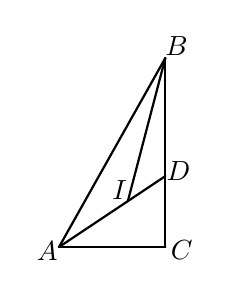
\begin{tikzpicture}[line cap=round,line join=round,>=triangle 45,x=1cm,y=1cm,scale=0.15]
                \draw [line width=0.8pt] (9,16)-- (9,0);
                \draw [line width=0.8pt] (0,0)-- (9,0);
                \draw [line width=0.8pt] (0,0)-- (9,16);
                \draw [line width=0.8pt] (0,0)-- (9,6);
                \draw [line width=0.8pt] (9,16)-- (5.826243132650954,3.8841620884339694);
                \begin{scriptsize}
                    \draw [fill=black] (9,0) circle (1pt);
                    \draw [fill=black] (9,16) circle (1pt);
                    \draw [fill=black] (0,0) circle (1pt);
                    \draw [fill=black] (9,6) circle (1pt);
                    \draw [fill=black] (5.826243132650954,3.8841620884339694) circle (1pt);
                \end{scriptsize}
                \draw[color=black] (10.385679024390247,-0.23822243902439044) node {$C$};
                \draw[color=black] (9.94284,16.988189268292715) node {$B$};
                \draw[color=black] (-0.995866341463415,-0.38106146341463465) node {$A$};
                \draw[color=black] (10.114246829268296,6.3895082926829385) node {$D$};
                \draw[color=black] (5.129076097560978,4.846922926829276) node {$I$};
            \end{tikzpicture}
    }
    \end{minipage}
    
    \question $a=\frac{501}{1001}$,$b=\frac{1001}{2001}$,$c=\frac{501+1001}{1001+2001}$,比較$a$、$b$、$c$的大小關係(由小到大)
    
    \question $a$、$b$、$c$、$d$為實數,已知多項式$1+cx^3+dx^4$可分解為$(1+2x)(1+ax)(1+bx)$,則$d=$?
    
    \question
    \begin{minipage}[t]{0.69\linewidth}
        如右圖,已知$\angle A=\ang{70}$,$\angle C=\ang{80}$,則$\angle B+\angle D+\angle E+\angle F+\angle G$為多少度?
    \end{minipage}
    \hfill
    \begin{minipage}[t]{0.3\linewidth}
        \adjustbox{valign=t, center}{
            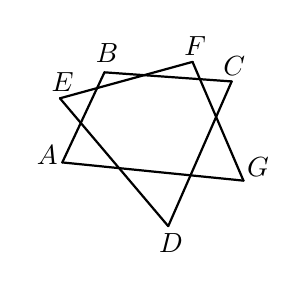
\begin{tikzpicture}[line cap=round,line join=round,>=triangle 45,x=1cm,y=1cm,scale=0.15]
                \draw [line width=0.8pt] (-4.61252,8.746352195121966)-- (-1.041544390243903,16.373956097561006);
                \draw [line width=0.8pt] (-1.041544390243903,16.373956097561006)-- (9.72851804878049,15.602625365853687);
                \draw [line width=0.8pt] (9.72851804878049,15.602625365853687)-- (4.357770731707318,3.3470370731707377);
                \draw [line width=0.8pt] (4.357770731707318,3.3470370731707377)-- (-4.812494634146343,14.174235121951245);
                \draw [line width=0.8pt] (-4.812494634146343,14.174235121951245)-- (6.414652682926831,17.25955804878052);
                \draw [line width=0.8pt] (6.414652682926831,17.25955804878052)-- (10.728391219512199,7.20369073170733);
                \draw [line width=0.8pt] (10.728391219512199,7.20369073170733)-- (-4.61252,8.746352195121966);
                \begin{scriptsize}
                    \draw [fill=black] (-4.61252,8.746352195121966) circle (1pt);
                    \draw [fill=black] (-1.041544390243903,16.373956097561006) circle (1pt);
                    \draw [fill=black] (9.72851804878049,15.602625365853687) circle (1pt);
                    \draw [fill=black] (4.357770731707318,3.3470370731707377) circle (1pt);
                    \draw [fill=black] (-4.812494634146343,14.174235121951245) circle (1pt);
                    \draw [fill=black] (6.414652682926831,17.25955804878052) circle (1pt);
                    \draw [fill=black] (10.728391219512199,7.20369073170733) circle (1pt);
                \end{scriptsize}
                \draw[color=black] (-5.883977560975611,9.36056) node {$A$};
                \draw[color=black] (-0.8130019512195126,17.988163902439055) node {$B$};
                \draw[color=black] (9.957060487804881,16.916833170731736) node {$C$};
                \draw[color=black] (4.586313170731708,1.9612448780487877) node {$D$};
                \draw[color=black] (-4.583952195121952,15.588442926829294) node {$E$};
                \draw[color=black] (6.643195121951222,18.57376585365857) node {$F$};
                \draw[color=black] (11.956933658536588,8.31789853658538) node {$G$};
            \end{tikzpicture}
        }
    \end{minipage}
    
    \question
    \begin{minipage}[t]{0.69\linewidth}
        如右圖,梯形$ABCD$中,$\overleftrightarrow{AB}\parallel\overleftrightarrow{CD}$,點$E$在$\overline{BC}$上,點$F$在$\overline{AD}$上,且$\overleftrightarrow{EF}\parallel\overleftrightarrow{AB}$。若$\overline{EF}:\overline{AB}=1:2$,$\overline{CE}:\overline{EB}=2:3$,梯形$ABEF$的面積為$54$,則梯形$ABCD$的面積為多少?
    \end{minipage}
    \hfill
    \begin{minipage}[t]{0.3\linewidth}
        \adjustbox{valign=t, center}{
            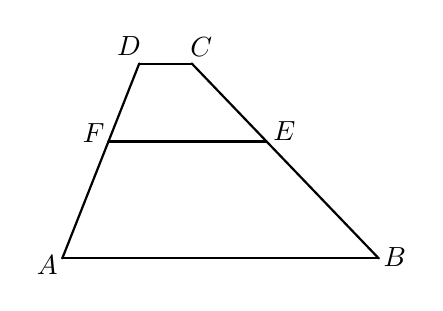
\begin{tikzpicture}[line cap=round,line join=round,>=triangle 45,x=1cm,y=1cm,scale=0.2]
                \draw [line width=0.8pt] (-5.898071219512197,2.8899521951219596)-- (14.185095609756102,2.8899521951219596);
                \draw [line width=0.8pt] (-2.969871219512196,10.303297560975631)-- (7.071712195121953,10.303297560975631);
                \draw [line width=0.8pt] (-1.0177378861788622,15.245527804878078)-- (2.329456585365854,15.245527804878078);
                \draw [line width=0.8pt] (-1.0177378861788622,15.245527804878078)-- (-5.898071219512197,2.8899521951219596);
                \draw [line width=0.8pt] (14.185095609756102,2.8899521951219596)-- (2.329456585365854,15.245527804878078);
                \begin{scriptsize}
                    \draw [fill=black] (-5.898071219512197,2.8899521951219596) circle (1pt);
                    \draw [fill=black] (14.185095609756102,2.8899521951219596) circle (1pt);
                    \draw [fill=black] (-2.969871219512196,10.303297560975631) circle (1pt);
                    \draw [fill=black] (7.071712195121953,10.303297560975631) circle (1pt);
                    \draw [fill=black] (-1.0177378861788622,15.245527804878078) circle (1pt);
                    \draw [fill=black] (2.329456585365854,15.245527804878078) circle (1pt);
                \end{scriptsize}
                \draw[color=black] (-6.855105365853661,2.4899648780487953) node {$A$};
                \draw[color=black] (15.213587317073175,2.961295609756114) node {$B$};
                \draw[color=black] (-3.912646829268294,10.846085853658565) node {$F$};
                \draw[color=black] (8.200203902439027,10.96035707317076) node {$E$};
                \draw[color=black] (-1.6700614634146347,16.345426341463454) node {$D$};
                \draw[color=black] (2.929405853658537,16.2739941463415) node {$C$};
            \end{tikzpicture}
        }
    \end{minipage}
    
    \question 求方程式$\sqrt{4x-2}-\sqrt{2x}=1$的解$x=$?
    
    \question 任一整數的平方所得到的值皆稱為完全平方數,例如:$0$,$1$,$4$,$9$,$16$,$25$,$\cdots$,皆為完全平方數。已知$x$是完全平方數,$x+180$也是完全平方數,則滿足條件的$x$有多少個?
    
    \question 設$a$為實數,已知滿足方程式$|||x-1|-2|+a|=3$的$x$共有$5$個,則$a=$?
    
    \question
    \begin{minipage}[t]{0.69\linewidth}
        如右圖,$ABCD$為長方形,$\overline{BC}$之中點為$O$,以$\overline{BC}$為直徑作一半圓(落在長方形內部),點$E$在$\overline{CD}$上,且$\overleftrightarrow{AE}$與此半圓相切,已知$\overline{AO}=20$,$\overline{OE}=15$,則長方形$ABCD$的面積為多少?
    \end{minipage}
    \hfill
    \begin{minipage}[t]{0.3\linewidth}
        \adjustbox{valign=t, center}{
            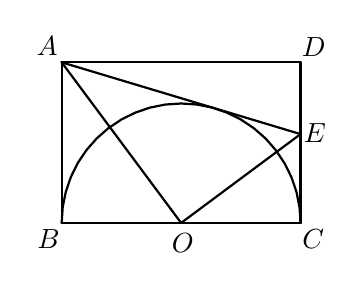
\begin{tikzpicture}[line cap=round,line join=round,>=triangle 45,x=1cm,y=1cm,scale=0.2]
                \draw [line width=0.8pt] (-6.06947804878049,8.032157073170756)-- (9.100026341463417,8.032157073170756);
                \draw [shift={(1.5152741463414636,8.032157073170756)},line width=0.8pt]  plot[domain=0:3.141592653589793,variable=\t]({1*7.584752195121954*cos(\t r)+0*7.584752195121954*sin(\t r)},{0*7.584752195121954*cos(\t r)+1*7.584752195121954*sin(\t r)});
                \draw [line width=0.8pt] (-6.06947804878049,18.23086341463419)-- (1.5152741463414636,8.032157073170756);
                \draw [line width=0.8pt] (1.5152741463414636,8.032157073170756)-- (9.100026341463419,13.672918159458922);
                \draw [line width=0.8pt] (-6.06947804878049,18.23086341463419)-- (-6.06947804878049,8.032157073170756);
                \draw [line width=0.8pt] (-6.06947804878049,18.23086341463419)-- (9.100026341463417,18.23086341463419);
                \draw [line width=0.8pt] (9.100026341463417,18.23086341463419)-- (9.100026341463417,8.032157073170756);
                \draw [line width=0.8pt] (9.100026341463419,13.672918159458922)-- (-6.06947804878049,18.23086341463419);
                \begin{scriptsize}
                    \draw [fill=black] (-6.06947804878049,8.032157073170756) circle (1pt);
                    \draw [fill=black] (9.100026341463417,8.032157073170756) circle (1pt);
                    \draw [fill=black] (-6.06947804878049,18.23086341463419) circle (1pt);
                    \draw [fill=black] (9.100026341463417,18.23086341463419) circle (1pt);
                    \draw [fill=black] (1.5152741463414636,8.032157073170756) circle (1pt);
                    \draw [fill=black] (9.100026341463419,13.672918159458922) circle (1pt);
                \end{scriptsize}
                \draw[color=black] (-6.897944390243905,6.989406829268314) node {$B$};
                \draw[color=black] (9.899924878048784,6.989406829268314) node {$C$};
                \draw[color=black] (-6.983647804878051,19.245020487804922) node {$A$};
                \draw[color=black] (9.928492682926832,19.216452682926874) node {$D$};
                \draw[color=black] (1.6152614634146343,6.7322712195122175) node {$O$};
                \draw[color=black] (10.014196097560978,13.760001951219545) node {$E$};
            \end{tikzpicture}
        }
    \end{minipage}
    
    \question 設$a$為實數,已知$x$的方程式$ax^2-x+2=0$的兩個解為相異的正整數,則$a=$?
    
    \question 將$2$、$3$、$4$、$5$、$6$重新排序之後得到$a$、$b$、$c$、$d$、$e$,若希望能滿足條件:$1+a+b=b+c+d=d+e+1$,則這樣的序組$(a,b,c,d,e)$有多少組?
    
\end{questions}

\vspace{1cm}

\section{計算證明題:本大題共有兩題,請依題意將解答過程及最後結果寫在「答案卷」上正確題號之空格內,未詳列計算過程者不予計分。每題12分}

\begin{questions}
    \question 如下圖,正三角形$ABC$的外接圓上有一點$P$(位於$\arc{BC}$上),$\overleftrightarrow{AC}$與$\overleftrightarrow{BP}$交於點$E$,$\overleftrightarrow{AB}$與$\overleftrightarrow{CP}$交於點$F$。證明:$\overline{BC}^2=\overline{CE}\times \overline{BF}$。
    
    \hfill
    \adjustbox{valign=t}{
        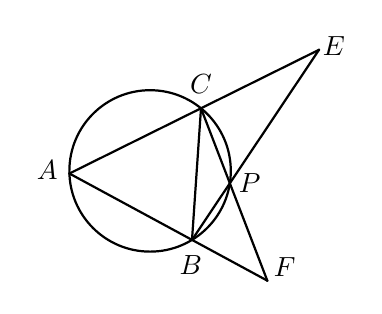
\begin{tikzpicture}[line cap=round,line join=round,>=triangle 45,x=1cm,y=1cm,scale=0.25]
            \draw [line width=0.8pt] (-1.2001027277606136,10.33599230658862) circle (4.100191944988989cm);
            \draw [line width=0.8pt] (-5.298147317073172,10.203310243902466)-- (7.382429970070207,16.489408386247064);
            \draw [line width=0.8pt] (7.382429970070207,16.489408386247064)-- (0.9296341463414635,6.832309268292705);
            \draw [line width=0.8pt] (-5.298147317073172,10.203310243902466)-- (4.755506476243252,4.761424245685313);
            \draw [line width=0.8pt] (4.755506476243252,4.761424245685313)-- (1.386719024390244,13.517175609756132);
            \draw [line width=0.8pt] (1.386719024390244,13.517175609756132)-- (0.9296341463414635,6.832309268292705);
            \begin{scriptsize}
                \draw [fill=black] (-5.298147317073172,10.203310243902466) circle (1pt);
                \draw [fill=black] (0.9296341463414635,6.832309268292705) circle (1pt);
                \draw [fill=black] (1.386719024390244,13.517175609756132) circle (1pt);
                \draw [fill=black] (2.8518818046891408,9.70909890692602) circle (1pt);
                \draw [fill=black] (7.382429970070207,16.489408386247064) circle (1pt);
                \draw [fill=black] (4.755506476243252,4.761424245685313) circle (1pt);
            \end{scriptsize}
            \draw[color=black] (-6.422834576325863,10.403701297356598) node {$A$};
            \draw[color=black] (0.8649284869901184,5.532051816698197) node {$B$};
            \draw[color=black] (1.3822834551153724,14.768408790764899) node {$C$};
            \draw[color=black] (3.8586453148664906,9.705272090387504) node {$P$};
            \draw[color=black] (8.133765789149937,16.66369641167218) node {$E$};
            \draw[color=black] (5.636577967648515,5.437093603354154) node {$F$};
        \end{tikzpicture}
    }
    
    \question 在坐標平面上,$X$軸的正向為東方,負向為西方;$Y$軸的正向為北方,負向為南方。一隻青蛙自原點$(0,0)$出發,依下列規則移動:
    \begin{enumerate}[label=(\arabic*)]
        \item 第一次可選擇「向東移動$2$單位」或「向西移動$1$單位」
        \item 若前一次向東移動$2$單位,則下一次只能「向北移動一單位」,若前一次向西移動$1$單位,則下一次只能「向南移動一單位」
        \item 若前一次向北或向南移動,則下一次只能向東西方向移動,但可自由選擇「向東移動$2$單位」或「向西移動$1$單位」
    \end{enumerate}
    證明:若此青蛙經$n$次移動之後回到坐標原點($n$為正整數),則$n$必等於$5$。
\end{questions}
    
\end{document}
